
\documentclass[border=20pt,preview]{standalone}
\usepackage{tikz}
\usepackage{xcolor}

\begin{document}

\begin{center}
    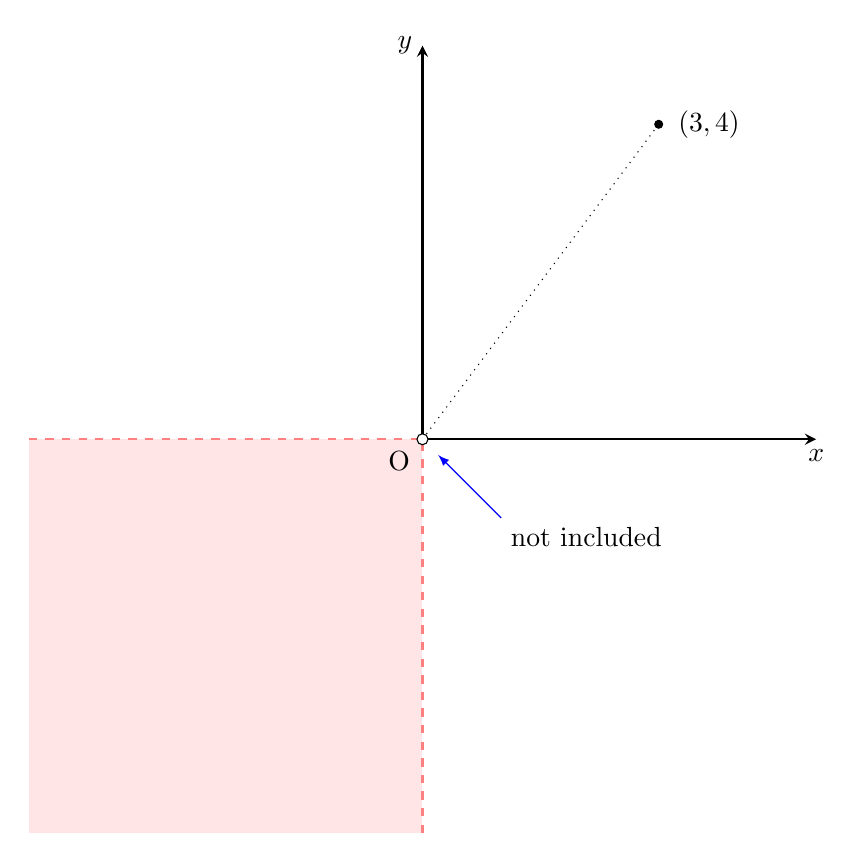
\begin{tikzpicture}
        \pgfmathsetmacro{\axislimit}{5}
        \fill[fill=red!10] (-\axislimit, 0) -- (0, 0) -- (0, -\axislimit) -- (-\axislimit, -\axislimit);

        \node[below left=1pt] (origin) at (0,0) {\(\rm{O}\)};
        \draw [-stealth,thick] (0, 0) -- (\axislimit, 0) node[below] {\(x\)};
        \draw [-stealth,thick] (0, 0) -- (0, \axislimit) node[left] {\(y\)};
        \draw [dashed,thick,draw=red!50] (0, -\axislimit) -- (0, 0);
        \draw [dashed,thick,draw=red!50] (-\axislimit, 0) -- (0, 0);

        \node (point) at (3, 4) {};
        \filldraw[fill=black] (point) circle (0.05);
        \node [right] at (point.east) {\((3, 4)\)};

        \draw [dotted] (0, 0) -- (3, 4);
        \filldraw[fill=white] (0, 0) circle (0.07);

        \draw[->,>=latex,draw=blue] (1, -1) node[below right] {not included} -- (0.2, -0.2);
    \end{tikzpicture}
\end{center}

\begin{center}
    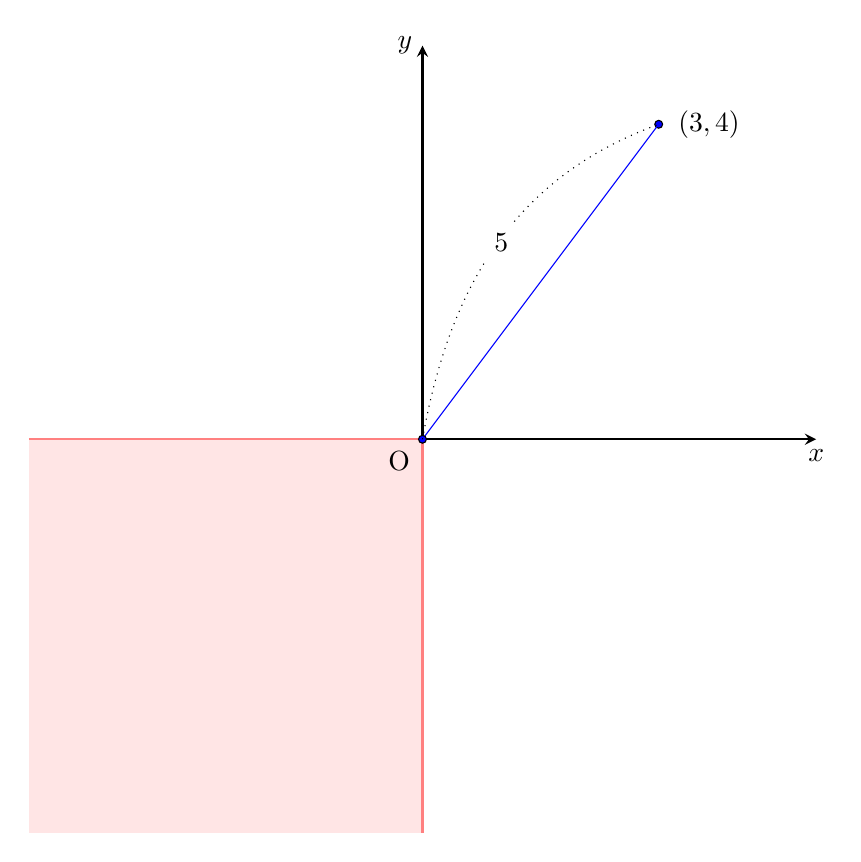
\begin{tikzpicture}
        \pgfmathsetmacro{\axislimit}{5}
        \fill[fill=red!10] (-\axislimit, 0) -- (0, 0) -- (0, -\axislimit) -- (-\axislimit, -\axislimit);

        \node[below left=1pt] (origin) at (0,0) {\(\rm{O}\)};
        \draw [-stealth,thick] (0, 0) -- (\axislimit, 0) node[below] {\(x\)};
        \draw [-stealth,thick] (0, 0) -- (0, \axislimit) node[left] {\(y\)};
        \draw [thick,draw=red!50] (0, -\axislimit) -- (0, 0);
        \draw [thick,draw=red!50] (-\axislimit, 0) -- (0, 0);

        \node (point) at (3, 4) {};
        \filldraw[fill=blue] (point) circle (0.05);
        \node [right] at (point.east) {\((3, 4)\)};

        \draw [blue] (0, 0) -- (3, 4);
        \filldraw[fill=blue] (0, 0) circle (0.05);
        \draw [dotted] (0, 0) to[out=80,in=-160] (3, 4);
        \node [fill=white] at (1, 2.5) {\(5\)};
    \end{tikzpicture}
\end{center}

\begin{center}
    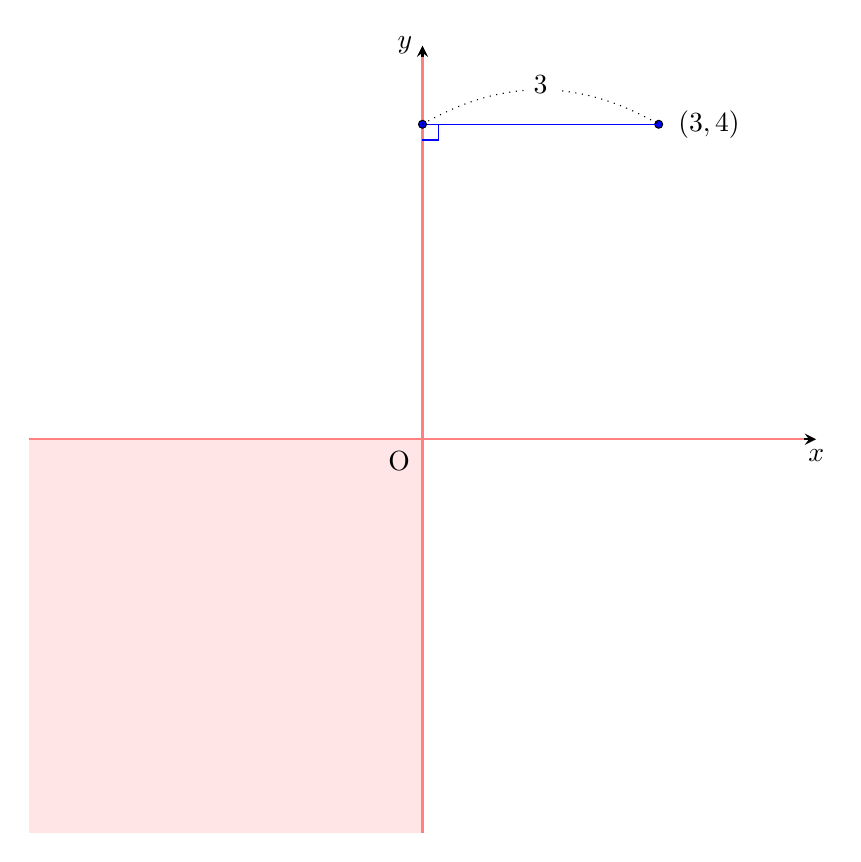
\begin{tikzpicture}
        \pgfmathsetmacro{\axislimit}{5}
        \fill[fill=red!10] (-\axislimit, 0) -- (0, 0) -- (0, -\axislimit) -- (-\axislimit, -\axislimit);

        \node[below left=1pt] (origin) at (0,0) {\(\rm{O}\)};
        \draw [-stealth,thick] (0, 0) -- (\axislimit, 0) node[below] {\(x\)};
        \draw [-stealth,thick] (0, 0) -- (0, \axislimit) node[left] {\(y\)};
        \draw [thick,draw=red!50] (0, -\axislimit) -- (0, \axislimit - 0.15);
        \draw [thick,draw=red!50] (-\axislimit, 0) -- (\axislimit - 0.15, 0);

        \node (point) at (3, 4) {};
        \filldraw[fill=blue] (point) circle (0.05);
        \node [right] at (point.east) {\((3, 4)\)};

        \draw [blue] (0, 4) -- (3, 4);
        \filldraw[fill=blue] (0, 4) circle (0.05);
        \draw [dotted] (0, 4) to[out=30,in=150] (3, 4);
        \node [fill=white] at (1.5, 4.5) {\(3\)};
        \draw [draw=blue] (0.2, 4) -- (0.2, 3.8) -- (0, 3.8);
    \end{tikzpicture}
\end{center}

\end{document}
